\documentclass[11pt, a4paper]{article}
\usepackage[utf8]{inputenc}
\usepackage{amsmath,setspace,geometry}
\usepackage{amsthm}
\usepackage{amsfonts}
\usepackage[shortlabels]{enumitem}
\usepackage{rotating}
\usepackage{pdflscape}
\usepackage{graphicx}
\usepackage{bbm}
\usepackage[dvipsnames]{xcolor}
\usepackage{hyperref}
\hypersetup{colorlinks=true, linkcolor= BrickRed, citecolor = BrickRed, filecolor = BrickRed, urlcolor = BrickRed, hypertexnames = true}
\usepackage[]{natbib} 
\bibpunct[:]{(}{)}{,}{a}{}{,}
\geometry{left = 1.0in,right = 1.0in,top = 1.0in,bottom = 1.0in}
\usepackage[english]{babel}
\usepackage{float}
\usepackage{caption}
\usepackage{subcaption}
\usepackage{booktabs}
\usepackage{pdfpages}
\usepackage{threeparttable}
\usepackage{lscape}
\usepackage{bm}
\setstretch{1.4}
%\usepackage[tablesfirst,nolists]{endfloat}

\newtheorem{theorem}{Theorem}
\newtheorem{assumption}{Assumption}
\newtheorem{lemma}{Lemma}
\newtheorem{definition}{Definition}
\newtheorem{proposition}{Proposition}
\newtheorem{claim}{Claim}
\newtheorem{corollary}{Corollary}
\newtheorem{example}{Example}
\DeclareMathOperator{\rank}{rank}


\title{Finite Sample Performance for Conduct Parameter Estimation in Homogenous Good Markets: Testing Perfect Competition is Difficult with 1000 Markets.}
\author{Yuri Matsumura\thanks{Department of Economics, Rice University. Email: Yuri.Matsumura@rice.edu} \and Suguru Otani \thanks{Department of Economics, Rice University. Email: so19@rice.edu
%Declarations of interest: none %this is for Economics Letters
}}

\begin{document}

\maketitle
\begin{abstract}
    We investigate finite sample performance for conduct parameter estimation. The statistical power increases when ; (1) the number of markets is large, (2) the conduct parameter is large, (3) when the rotation instrument is strong. We find that rejecting the null hypothesis that markets are given by perfect competition is difficult even when the number of markets is moderate, e.g. 1000 and the number of firms is five regardless of the strength of instruments.
\vspace{0.1in}

\noindent\textbf{Keywords:} Conduct parameters, Homogenous goods market, Monte Carlo simulation
\vspace{0in}
\newline
\noindent\textbf{JEL Codes:} C5, C13, L1

\bigskip
\end{abstract}


\section{Introduction}
Measuring competitiveness is an important task in the empirical industrial organization literature.
A conduct parameter is considered to be a useful measure of competitiveness. 
However, the parameter cannot be directly measured from data because data generally lack information about marginal costs.
Therefore, researchers endeavor to learn conduct parameters.

Researchers both estimate and test structural models to learn firm conduct.
We focus on homogenous good markets.\footnote{See \cite{nevoIdentificationOligopolySolution1998}, \cite{magnolfi2022comparison}, and \cite{duarte2023testing} for the case of differentiated goods markets.}
For estimation of conduct parameters, \citet{bresnahan1982oligopoly} considers identification of conduct parameters for the linear model. \cite{matsumura2023resolving} resolves the conflict on some identification problems between \cite{bresnahan1982oligopoly} and \cite{perloff2012collinearity}. \cite{matsumura2023mpec} show the importance of equilibrium existence conditions of the log-linear model. 
For testing conduct parameters, \cite{genesove1998testing} estimate and test conduct parameters, then compare these with direct measures using actual marginal cost data of the U.S. sugar industry. 
They show that perfect competition cannot be rejected when market power is around 0.1 and the number of markets is less than 100.
\cite{corts1999conduct} argues that the conduct parameter fails to measure and test market power accurately if firms consider dynamic features in a repeated game.

Although conduct parameter estimation and testing are one of the most popular but controversial approaches in the literature, to the best of our knowledge, there is no paper conducting formal Monte Carlo simulations. 
To fill in the gap between conceptual discussion and empirical performance, we investigate finite sample performance of conduct parameter estimation of homogeneous good markets. 
Concretely, we conduct a statistical power analysis varying the number of markets, firms, and strength of demand rotation instruments under the null hypothesis that markets are given by perfect competition.

We find that the power increases when ; (1) sample size is large, that is, the number of markets is large, (2) the conduct parameter is large, (3) when the rotation instrument is strong. 
As a remarkable finding is that the rejection frequency cannot achieve 90\% when the number of markets is moderate, e.g. 1000, and the number of firms is five regardless of the strength of instruments. 
This confirms that the testing problem 
 of \cite{genesove1998testing} caused by the small number of markets.

Our results and code provide a unified reference for applied researchers to consider the feasibility to test the assumption on firm conduct, i.e., homogenous good markets are assumed to be perfect competition, Cournot competition, or perfect collusion.

\section{Model}
Consider data with $M$ markets with homogeneous products.
Assume that there are $N$ firms in each market.
Let $m = 1,\ldots, M$ be the index for markets.
Then, we obtain a supply equation as follows:
\begin{align}
     P_m = -\theta\frac{\partial P_m(Q_{m})}{\partial Q_{m}}Q_{m} + MC_m(Q_{m}),\label{eq:supply_equation}
\end{align}
where $Q_{m}$ is the aggregate quantity, $P_m(Q_{m})$ is the demand function, $MC_{m}(Q_{m})$ is the marginal cost function, and $\theta\in[0,1]$ is  the conduct parameter. 
The equation nests perfect competition ($\theta=0$), Cournot competition ($\theta=1/N$), and perfect collusion ($\theta=1$).\footnote{See \cite{bresnahan1982oligopoly}.} 

Consider an econometric model that integrates the above model.
Assume that the demand and marginal cost functions are written as follows: 
\begin{align}
    P_m = f(Q_{m}, Y_m, \varepsilon^{d}_{m}, \alpha), \label{eq:demand}\\
    MC_m = g(Q_{m}, W_{m}, \varepsilon^{c}_{m}, \gamma),\label{eq:marginal_cost}
\end{align}
where $Y_m$ and $W_{m}$ are vectors of exogenous variables, $\varepsilon^{d}_{m}$ and $\varepsilon^{c}_{m}$ are error terms, and $\alpha$ and $\gamma$ are vectors of parameters.
Additionally, we have demand- and supply-side instrumental variables, $Z^{d}_{m}$ and $Z^{c}_{m}$, and assume that the error terms satisfy the mean independence conditions, $E[\varepsilon^{d}_{m}\mid Y_m, Z^{d}_{m}] = E[\varepsilon^{c}_{m} \mid W_{m}, Z^{c}_{m}] =0$.

\subsection{Linear demand and cost}
Assume that linear demand and marginal cost functions are specified as follows:
\begin{align}
    P_m &= \alpha_0 - (\alpha_1 + \alpha_2Z^{R}_{m})Q_{m} + \alpha_3 Y_m + \varepsilon^{d}_{m},\label{eq:linear_demand}\\
    MC_m &= \gamma_0  + \gamma_1 Q_{m} + \gamma_2 W_{m} + \gamma_3 R_{m} + \varepsilon^{c}_{m},\label{eq:linear_marginal_cost}
\end{align}
where $W_{m}$ and $R_{m}$ are excluded cost shifters and $Z^{R}_{m}$ is Bresnahan's demand rotation instrument. 
The supply equation is written as follows:
\begin{align}
    P_m 
    %&= \gamma_0 + [\theta(\alpha_1 + \alpha_2Z^{R}_{m})+ \gamma_1] Q_{m}   + \gamma_2 W_{m} + \gamma_3 R_{m} + \varepsilon^{c}_{m}\nonumber\\ 
    &= \gamma_0 + \theta \alpha_2 Z^{R}_mQ_{m} + (\theta\alpha_1 + \gamma_1) Q_{m} + \gamma_2 W_m + \gamma_3 R_{m} +\varepsilon^c_m.\label{eq:linear_supply_equation}
\end{align}
By substituting Equation \eqref{eq:linear_demand} with Equation \eqref{eq:linear_supply_equation} and solving it for $P_m$, we obtain the aggregate quantity $Q_{m}$ based on the parameters and exogenous variables as follows:
\begin{align}
    Q_{m} =  \frac{\alpha_0 + \alpha_3 Y_m - \gamma_0 - \gamma_2 W_{m} - \gamma_3 R_{m} + \varepsilon^{d}_{m} - \varepsilon^{c}_{m}}{(1 + \theta) (\alpha_1 + \alpha_2 Z^{R}_{m}) + \gamma_1}.\label{eq:quantity_linear}
\end{align}


\section{Simulation results}\label{sec:results}

\subsection{Simulation and estimation procedure}

We set true parameters and distributions as shown in Table \ref{tb:parameter_setting}. 
We vary the true value of $\theta$ from 0.05 (20-firms symmetric Cournot) to 1 (perfect collusion) and the strength of demand rotation instrument, $\alpha_2$, from 0.1 (weak) to 20.0 (extremely strong) which is unrealistically larger than the price coefficient, $\alpha_1$.
For simulation, we generate 100 data sets.
We separately estimate the demand and supply equation by using two-stage least squares (2SLS) estimation.
The instrumental variables for demand estimation are $Z^{d}_{m} = (Z^{R}_{m}, Y_m, H_{m}, K_{m})$ and the instrumental variables for supply estimation are $Z^{c}_{m} = (Z^{R}_{m}, W_{m}, R_{m}, Y_m)$. 

\begin{table}[!htbp]
    \caption{True parameters and distributions}
    \label{tb:parameter_setting}
    \begin{center}
    \subfloat[Parameters]{
    \begin{tabular}{cr}
            \hline
            & linear  \\
            $\alpha_0$ & $10.0$  \\
            $\alpha_1$ & $1.0$  \\
            $\alpha_2$ & $\{0.1,0.5,1.0,5.0,20.0\}$ \\
            $\alpha_3$ & $1.0$  \\
            $\gamma_0$ & $1.0$ \\
            $\gamma_1$ & $1.0$  \\
            $\gamma_2$ & $1.0$ \\
            $\gamma_3$ & $1.0$\\
            $\theta$ & $\{0.05,0.1,0.2,0.33,0.5,1.0\}$ \\
            \hline
        \end{tabular}
    }
    \subfloat[Distributions]{
    \begin{tabular}{crr}
            \hline
            & linear\\
            Demand shifter&  \\
            $Y_m$ & $N(0,1)$  \\
            Demand rotation instrument&   \\
            $Z^{R}_{m}$ & $N(10,1)$ \\
            Cost shifter&    \\
            $W_{m}$ & $N(3,1)$  \\
            $R_{m}$ & $N(0,1)$   \\
            $H_{m}$ & $W_{m}+N(0,1)$  \\
            $K_{m}$ & $R_{m}+N(0,1)$   \\
            Error&  &  \\
            $\varepsilon^{d}_{m}$ & $N(0,\sigma)$  \\
            $\varepsilon^{c}_{m}$ & $N(0,\sigma)$ \\
            \hline
        \end{tabular}
    }
    \end{center}
    \footnotesize
    Note: $\sigma=1.0$. $N:$ Normal distribution. $U:$ Uniform distribution.
\end{table}

Figure \ref{fg:theta_hat_power} presents the results of finite sample performance.\footnote{See online appendix for simulation details. See the author's github for the results of all other parameters.}
We focus on the power of conduct parameter $\theta$. 
The null hypothesis is that markets are given by perfect competition.
I compute the rejection
frequency as the power by using t-statistics at a significance level of 0.05 over 100 datasets.
The rejection
frequency increases when ; (1) sample size is large, that is, the number of markets is large, (2) $\theta$ is large, that is, the number of firms is smaller, (3) when $\alpha_2$ is large, that is, the rotation instrument is stronger.
Panel (f) shows that if the number of firms is twenty $(\theta=0.05)$, with enough large number of markets, will give us approximately 70\% power to reject the null hypothesis that markets are given by perfect competition.
As a remarkable finding is that the rejection frequency cannot achieve 90\% even when the number of markets is moderate, e.g. 1000 and the number of firms is five regardless of the strength of instruments. 
This confirms that the rejection problem 
 of \cite{genesove1998testing} caused by the small number of markets.


\begin{figure}[!ht]
  \begin{center}
  % \subfloat[M=50]{\includegraphics[width = 0.32\textwidth]
  % {figuretable/theta_hat_power_50.png}}
  \subfloat[$M=100$]{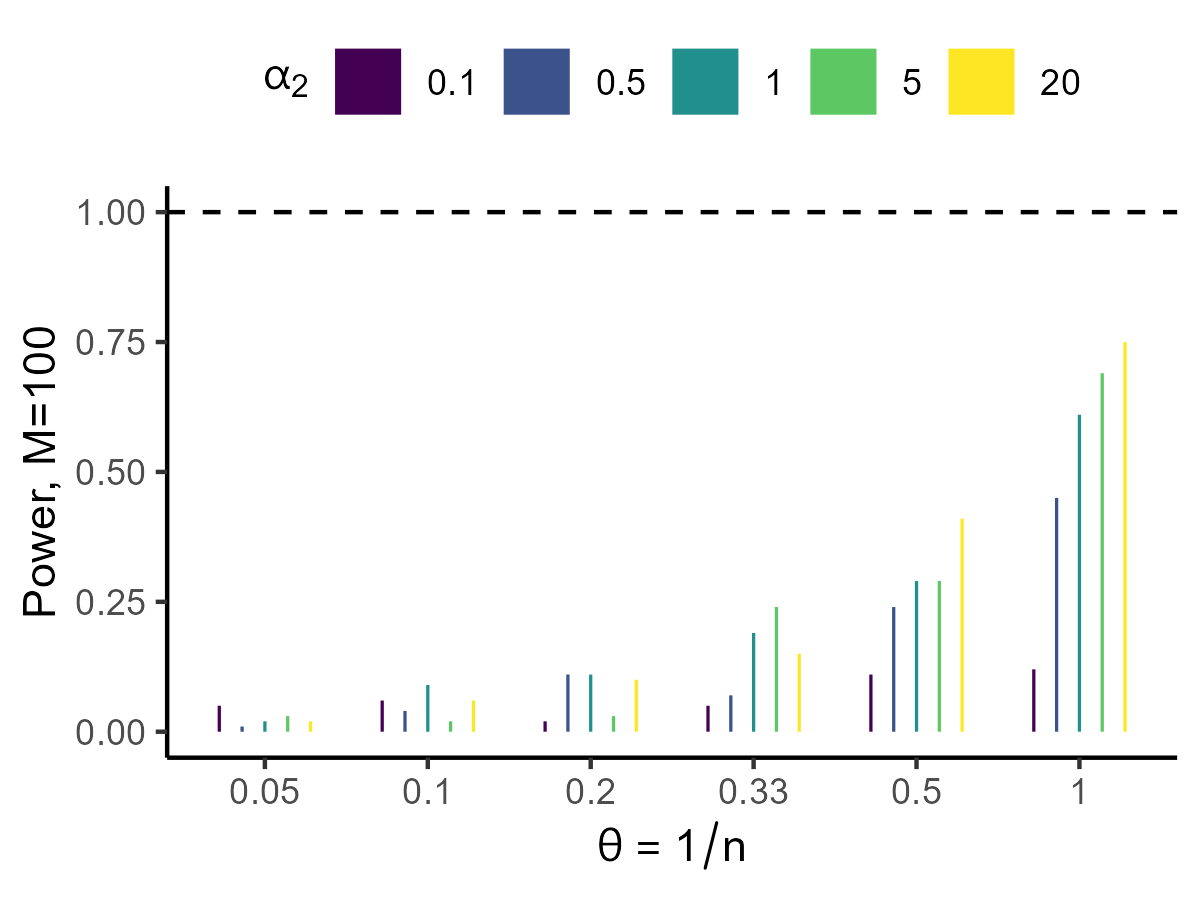
\includegraphics[width = 0.32\textwidth]
  {figuretable/theta_hat_power_100.png}}
  \subfloat[$M=200$]{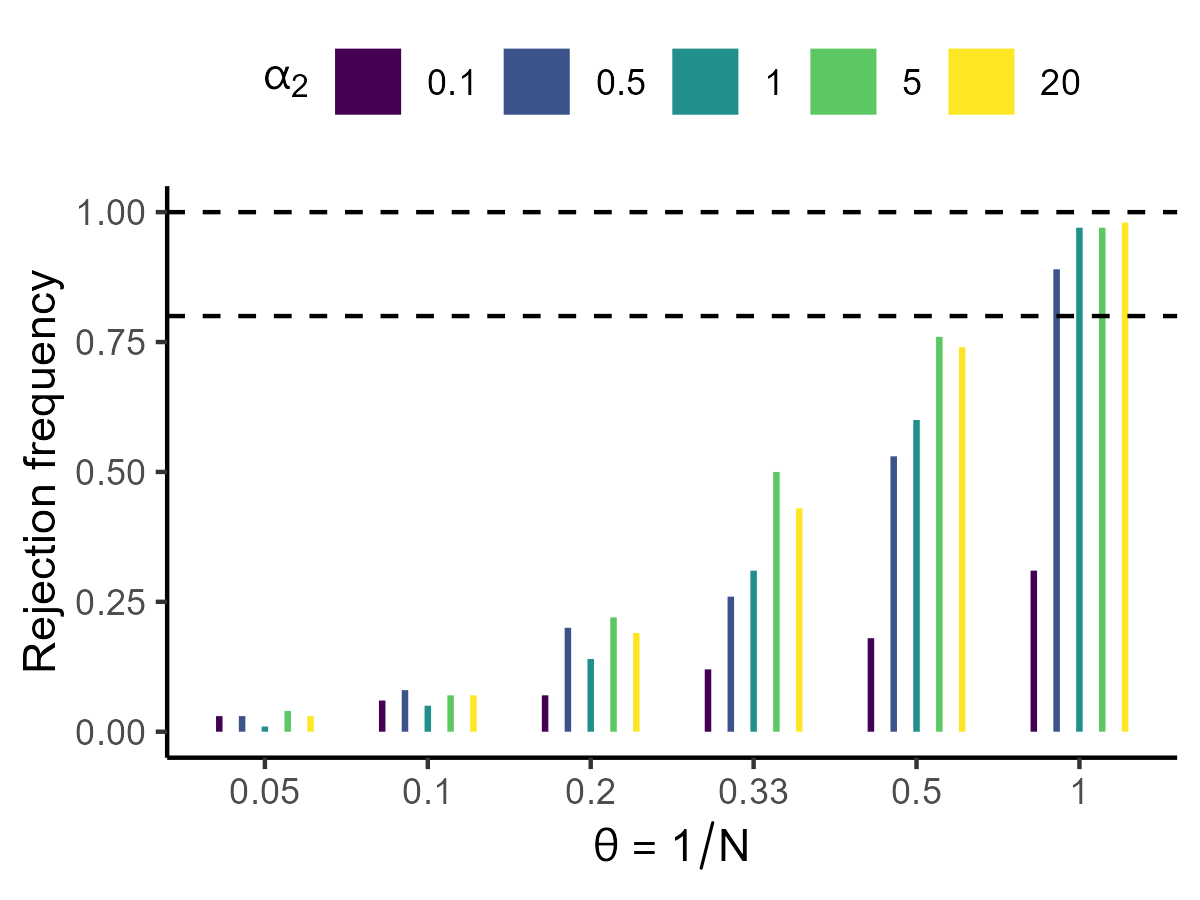
\includegraphics[width = 0.32\textwidth]
  {figuretable/theta_hat_power_200.png}}
  \subfloat[$M=1000$]{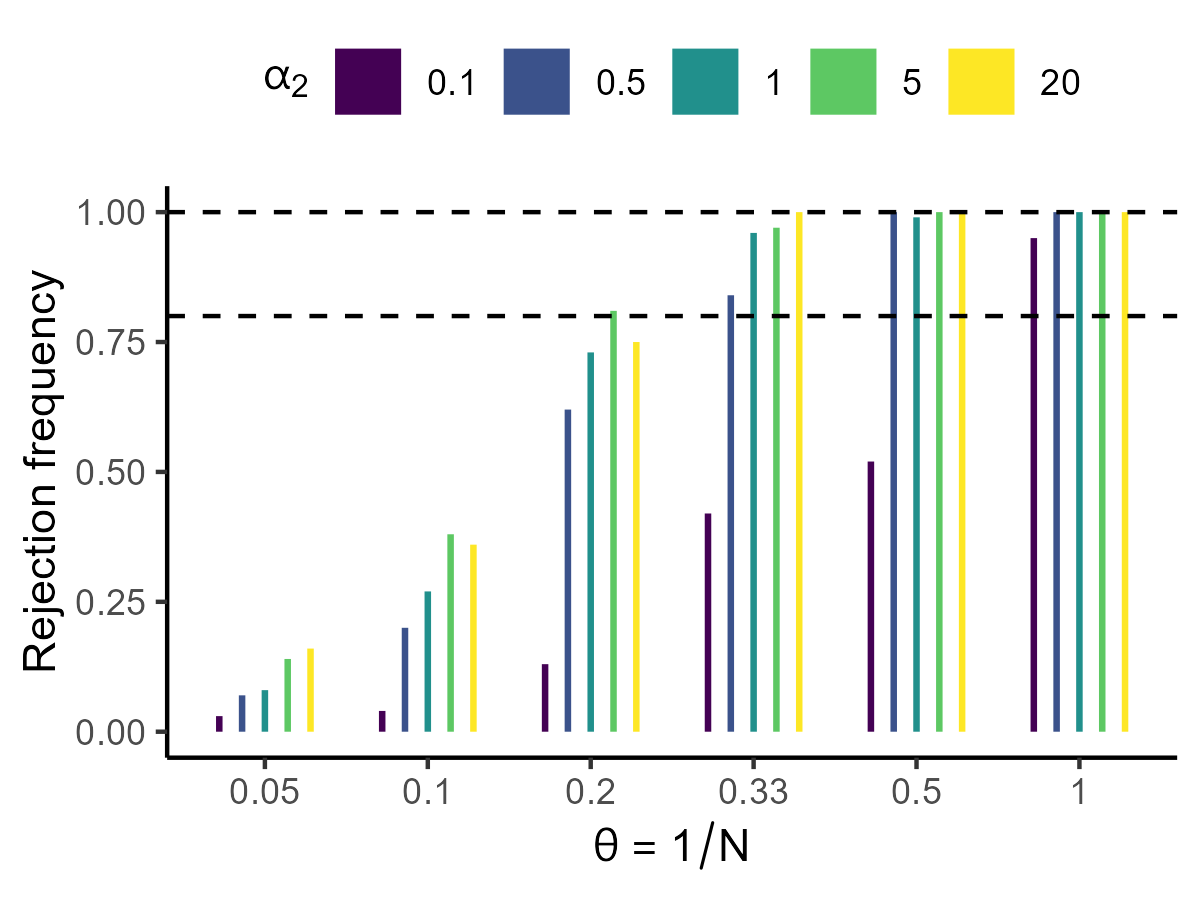
\includegraphics[width = 0.32\textwidth]
  {figuretable/theta_hat_power_1000.png}}\\
  \subfloat[$M=2000$]{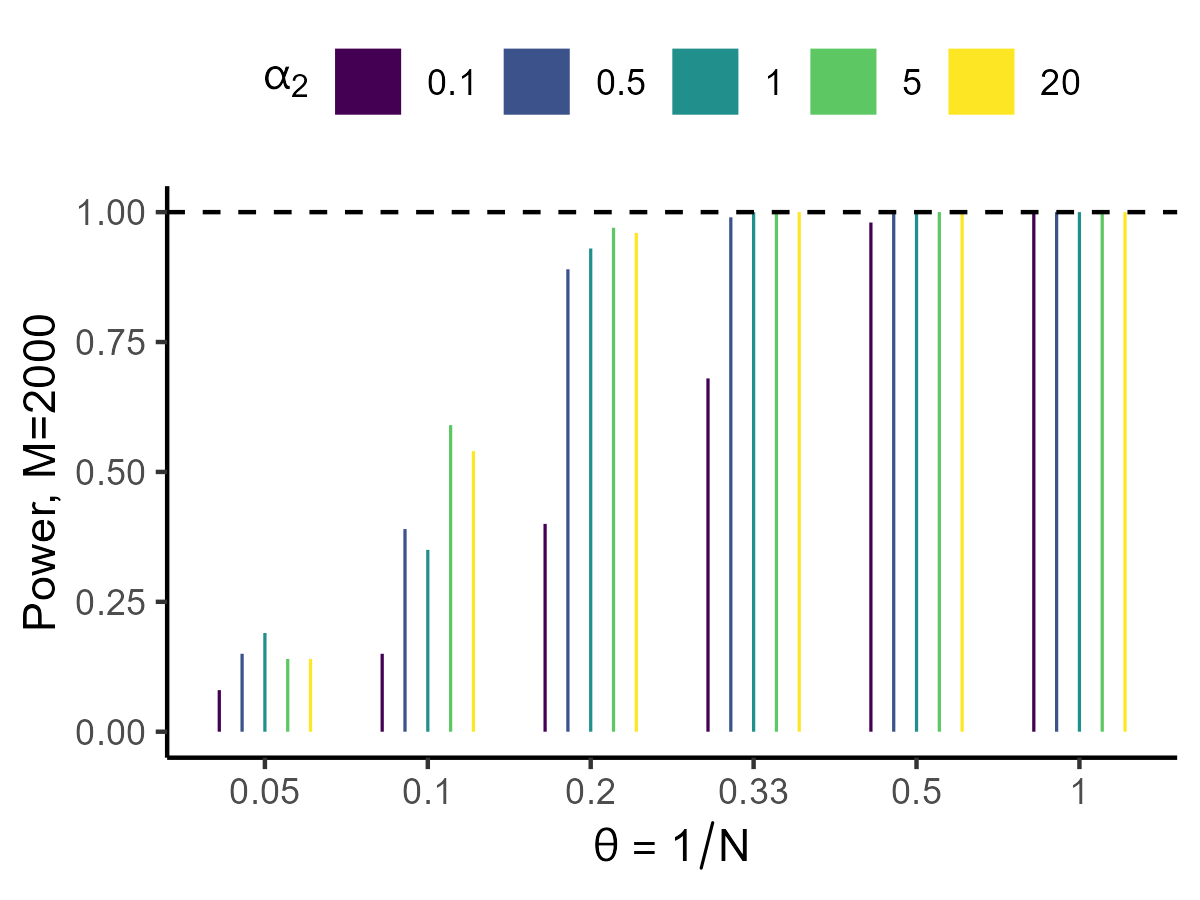
\includegraphics[width = 0.32\textwidth]
  {figuretable/theta_hat_power_2000.png}}
  \subfloat[$M=5000$]{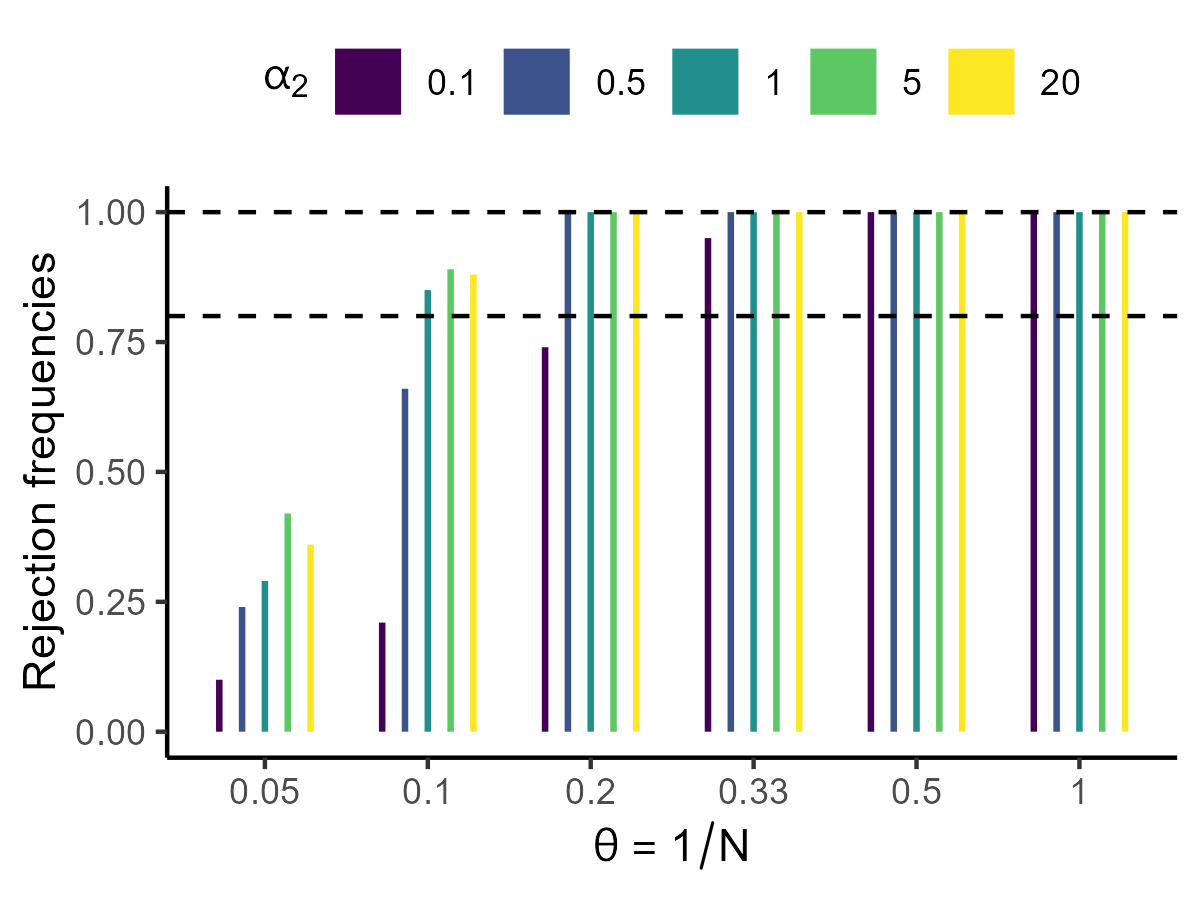
\includegraphics[width = 0.32\textwidth]
  {figuretable/theta_hat_power_5000.png}}
  \subfloat[$M=10000$]{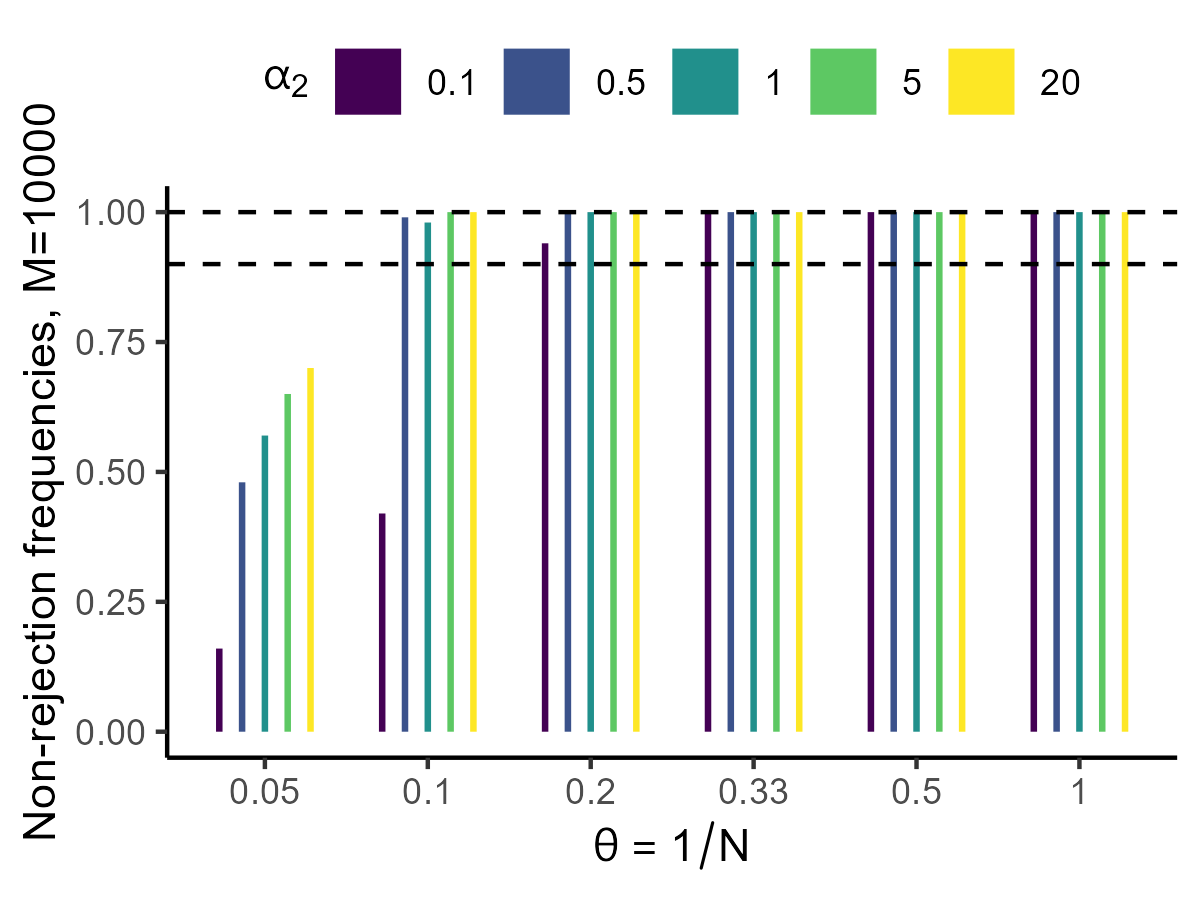
\includegraphics[width = 0.32\textwidth]
  {figuretable/theta_hat_power_10000.png}}
  \caption{Statistical power of conduct parameter $\theta$}
  \label{fg:theta_hat_power}
  \end{center}
  \footnotesize
   %Note: We simulate 100 datasets.
\end{figure} 



\section{Conclusion}

We conduct a statistical power analysis for conduct parameter estimation. The power increases when ; (1) sample size is large, that is, the number of markets is large, (2) the conduct parameter is large, (3) when the rotation instrument is strong. We find that rejecting the null hypothesis that markets are given by perfect competition is difficult even when the number of markets is moderate, e.g. 1000 and the number of firms is five regardless of the strength of instruments.


\paragraph{Acknowledgments}
We thank Jeremy Fox and Isabelle Perrigne for their valuable advice. This research did not receive any specific grant from funding agencies in the public, commercial, or not-for-profit sectors. 

\newpage


\bibliographystyle{aer}
\bibliography{conduct_parameter}

\newpage

\setcounter{page}{1}
\appendix
\section{Online appendix}\label{sec:appendix}




\subsection{Details for our simulation settings}

To generate the simulation data, for each model, we first generate the exogenous variables $Y_m, Z^{R}_{m}, W_m, R_{m}, H_m$, and $K_m$ and the error terms $\varepsilon_{m}^c$ and $\varepsilon_{m}^d$ based on the data generation process in Table \ref{tb:parameter_setting}.
We compute the equilibrium quantity $Q_{m}$ for the linear model by \eqref{eq:quantity_linear}.
We then compute the equilibrium price $P_m$ by substituting $Q_{m}$ and other variables into the demand function \eqref{eq:linear_demand}.

We estimate the equations using the \texttt{ivreg} package in \texttt{R}.
An important feature of the model is that we have an interaction term of the endogenous variable $Q_{m}$ and the instrumental variable $Z^{R}_{m}$.
The \texttt{ivreg} package automatically detects that the endogenous variables are $Q_{m}$ and the interaction term $Z^{R}_{m}Q_{m}$, running the first stage regression for each endogenous variable with the same instruments. To confirm this, we manually write R code to implement the 2SLS model. 
When the first stage includes only the regression of $Q_{m}$, estimation results from our code differ from the results from \texttt{ivreg}. 
However, when we modify the code to regress $Z^{R}_{m}Q_{m}$ on the instrument variables and estimate the second stage by using the predicted values of $Q_{m}$ and $Z^{R}_{m}Q_{m}$, the result from our code and the result from \texttt{ivreg} coincide.




\end{document}